\chapter{Projeto de implementação}
\label{cap:projetoimplementacao}

Neste capítulo será feito a identificação dos serviços mais críticos da empresa para posteriormente ser possível propor uma solução de 
implementação de alta disponibilidade desses serviços que são fornecidos pela empresa, sendo que eles foram detalhados no Capítulo 
\ref{cap:estudodecaso}. Com isso pretende-se atingir o objetivo deste trabalho.

\section{Levantamento dos serviços críticos}
\label{section:servcrit}

No capítulo anterior foram detalhados todos os serviços que estão disponíveis na empresa. Sendo assim, nesta seção será feito uma análise desses
serviços, destacando os serviços considerados mais críticos para a empresa. 

O principal objetivo da empresa sempre foi priorizar a estabilidade e qualidade dos serviços fornecidos pela mesma. Deste modo, será definido 
alguns critérios para possibilitar a identificação dos serviços mais críticos para a empresa. Esses critérios são:
\begin{itemize}
 \item A quantidade de clientes ou funcionários que utilizam o serviço: esse é o item mais relevante, pois impacta diretamente no faturamento
 da empresa. De fato, se um cliente ficar sem acesso à internet, o cliente terá um desconto proporcional, na sua fatura, ao tempo que ficou sem 
 acesso; 
 \item O número de requisições em um determinado tempo: esse número é importante, uma vez que, indicam a quantidade de usuários que dependem do 
 serviço. São exemplos dessa medida a quantidade de acessos por minuto em um servidor de hospedagens de sites e a quantidade de requisições 
 \ac{DNS} em um servidor recursivo;
 \item O volume de elementos do serviço: essa medida demonstra a abrangência do serviço, ou seja, quantos objetos existem em um serviço e 
 consequentemente quantos clientes são dependentes deste. Como, por exemplo, a quantidade de contas de \textit{e-mail} em um servidor de 
 \textit{e-mail} e a quantidade de equipamentos monitorados por um servidor de monitoramento. Esse critério é importante pois com ele pode-se
 comparar diferentes serviços possibilitando perceber o grau de relevância que cada um possui;
 \item O número de conexões \ac{TCP} ou o número de transmissões \ac{UDP}: essa medida pode demonstrar a quantidade de acessos simultâneos que um
 serviço pode atingir. Esse critério, como o anterior, também permite comparar diferentes serviços para ter a possibilidade de ordená-los de acordo 
 com sua relevância, por isso o torna importante para esta análise.
\end{itemize}

Considerando esses critérios, pode-se identificar os seguintes serviços:
\begin{itemize}
 \item \ac{DNS} recursivo primário: esse serviço foi classificado como o mais importante pois possui um impacto direto nos clientes do provedor. 
 Esse é o único serviço que todos os clientes e funcionários utilizam. O objetivo de um provedor é fornecer uma navegação de qualidade aos seus 
 clientes, sendo assim, o \ac{DNS} é fundamental para essa navegação. O primeiro critério desse serviço é a quantidade de clientes
 que ele possui, que é aproximadamente 9000. Outro importante critério que pode ser aplicado ao \ac{DNS} recursivo é o número de 
 requisições por segundo, que chega aproximadamente a 1150 (Figura \ref{fig:passata_week}). De acordo com a Figura \ref{fig:servico_udp}, que 
 compara os principais servidores da empresa através de transmissões \ac{UDP}, onde pode-se claramente perceber que o servidor \textit{Passata}
 possui um grande número de transmissões \ac{UDP}, o qual fornece o serviço de \ac{DNS} recursivo primário. 
 Assim, esse serviço se torna o maior entre todos os outros;
 
\begin{figure}[h!]
 \centering
 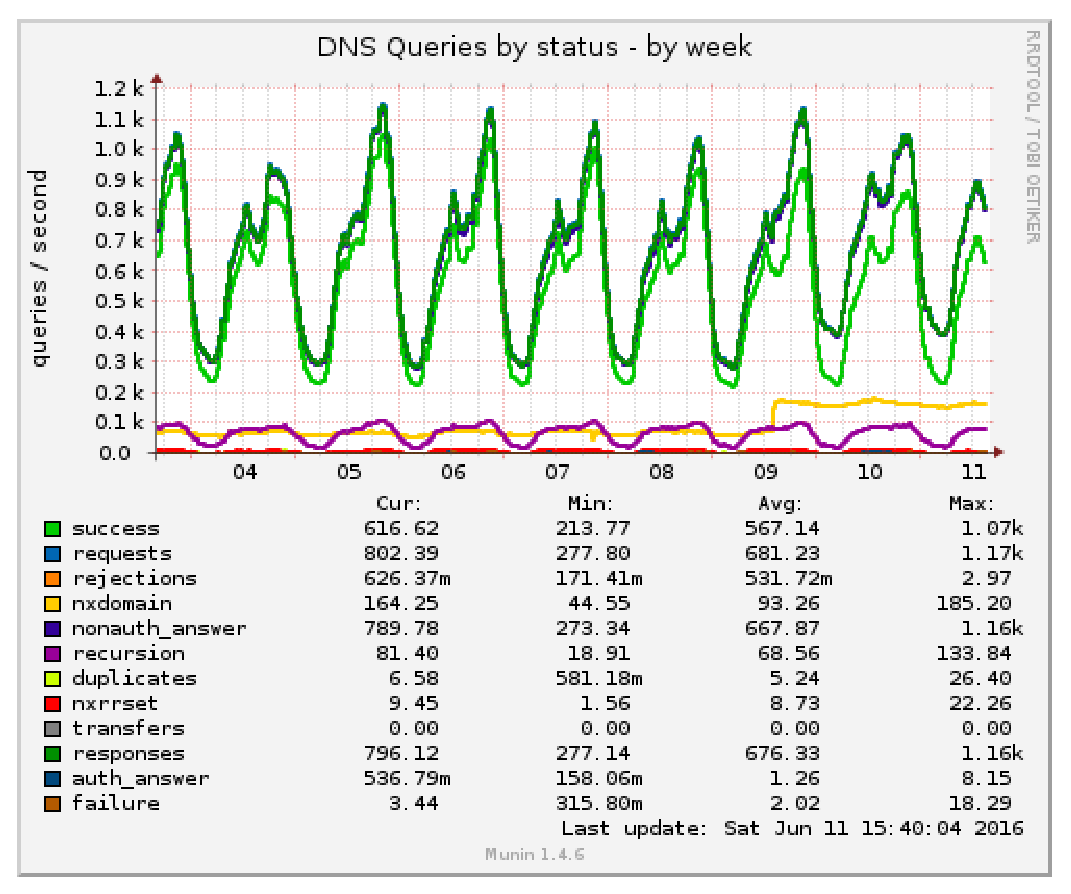
\includegraphics[width=310px]{img/passata_week.eps}
 \caption{Gráfico de requisições DNS.}
 \label{fig:passata_week}
\end{figure}

\begin{figure}[h!]
 \centering
 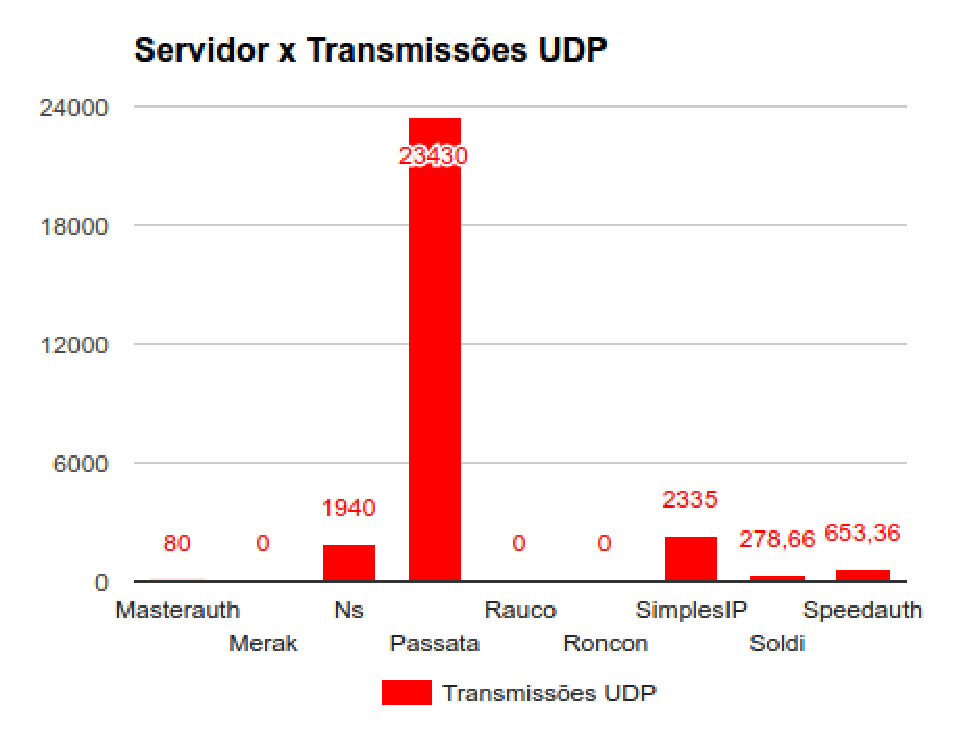
\includegraphics[width=430px]{img/servico_udp.eps}
 \caption{Gráfico de comparação de transmissões UDP entre os principais servidores.}
 \label{fig:servico_udp}
\end{figure}

 \item \textit{Radius}: esse serviço é importante para a navegação dos clientes do provedor, pois esse é o responsável pela autenticação de 
 todos os clientes. Caso esse serviço fique indisponível os clientes não conseguirão estabelecer conexão para navegação. Os servidores
 \textit{Speedauth} e \textit{Masterauth} recebem uma média de 1,6 requisições de autenticação por segundo como pode ser visto na Figura 
 \ref{fig:speedauth_auth_week} e na \ref{fig:masterauth_auth_week}, esse número se torna expressivo pois demonstra que a cada um segundo 
 aproximadamente um cliente requisita a autenticação para iniciar a sua navegação. Além disso, esse serviço armazena alguns dados relacionados 
 à conexão dos clientes, que são os seguintes dados: o endereço de \ac{IP} que é utilizado por um cliente em um determinado período, o tráfego 
 de dados da conexão, o tempo da conexão de cada cliente, o endereço \ac{MAC} dos equipamentos dos clientes, entre outros. Essas operações 
 resultam em um número de requisições por segundo (em média 23 requisições).
 %, como pode ser observado na Figura \ref{fig:speedauth_acct_week} e \ref{fig:masterauth_acct_week};
 Outro critério que é relevante para esses servidores é o volume de elementos do serviço, que neste caso, representa a quantidade de \textit{logins} 
 de autenticação dos clientes de acesso a internet do provedor. De acordo com a Figura \ref{fig:servico_elemento}, os servidores \textit{Speedauth} 
 e \textit{Masterauth} estão entre os maiores, sendo que essa figura compara os principais servidores da empresa através do volume de elementos
 que foi descrito no terceiro critério. Além disso, existe um destaque desses servidores no número de conexões \ac{TCP}, como pode ser observado 
 na Figura \ref{fig:servico_tcp};
 
\begin{figure}[h!]
 \centering
 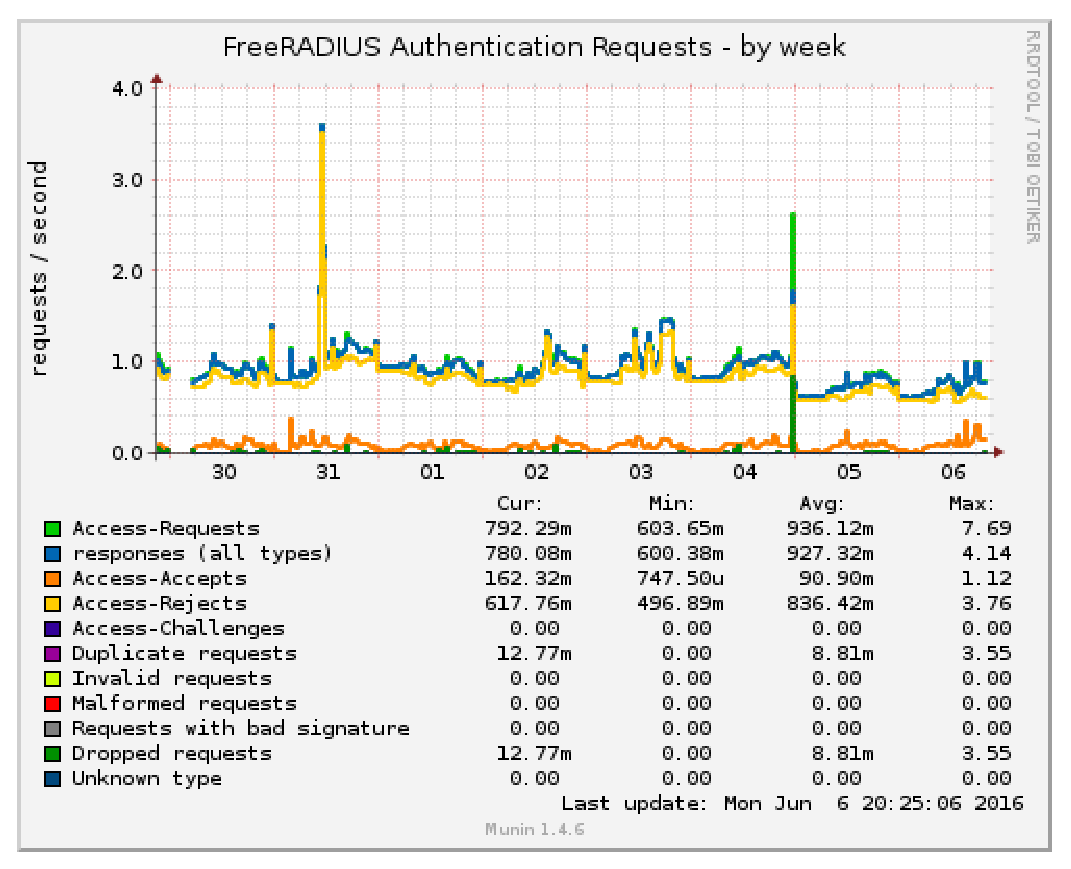
\includegraphics[width=310px]{img/speedauth_auth_week.eps}
 \caption{Gráfico de requisições de autenticação do servidor Speedauth.}
 \label{fig:speedauth_auth_week}
\end{figure}

\begin{figure}[h!]
 \centering
 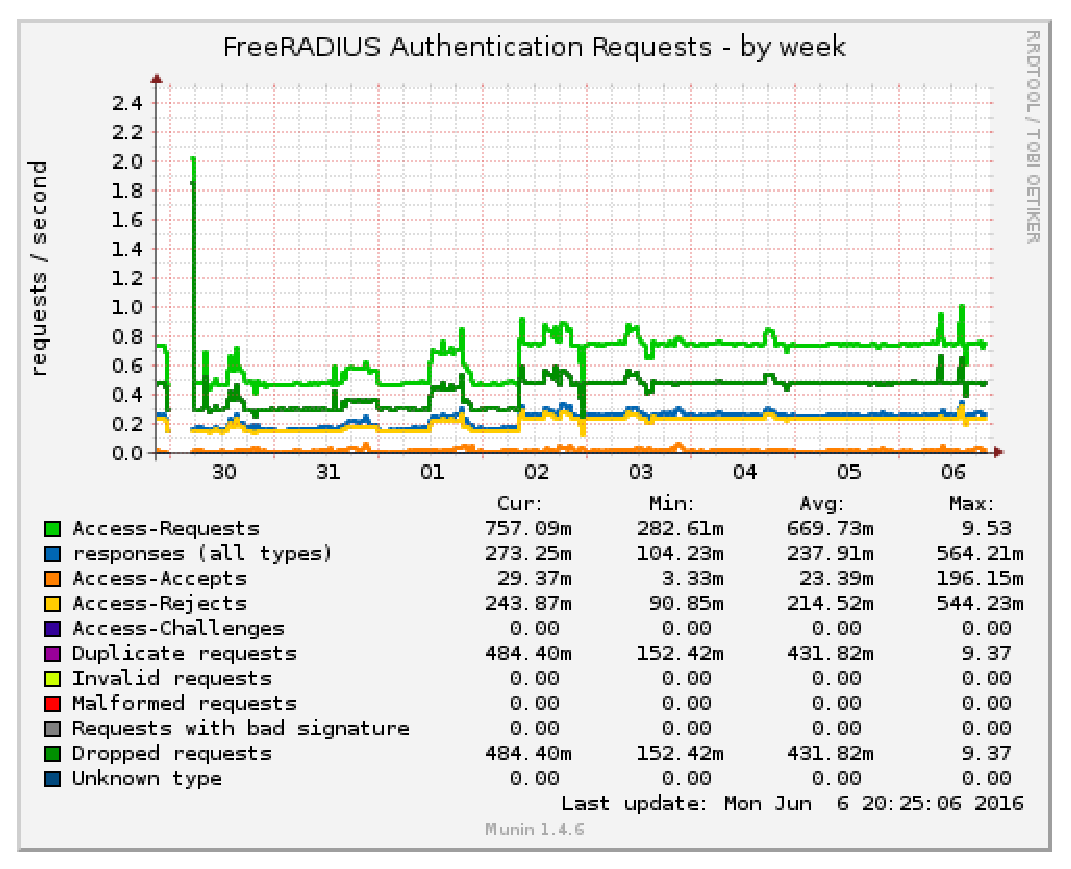
\includegraphics[width=310px]{img/masterauth_auth_week.eps}
 \caption{Gráfico de requisições de autenticação do servidor Masterauth.}
 \label{fig:masterauth_auth_week}
\end{figure}

\begin{figure}[h!]
 \centering
 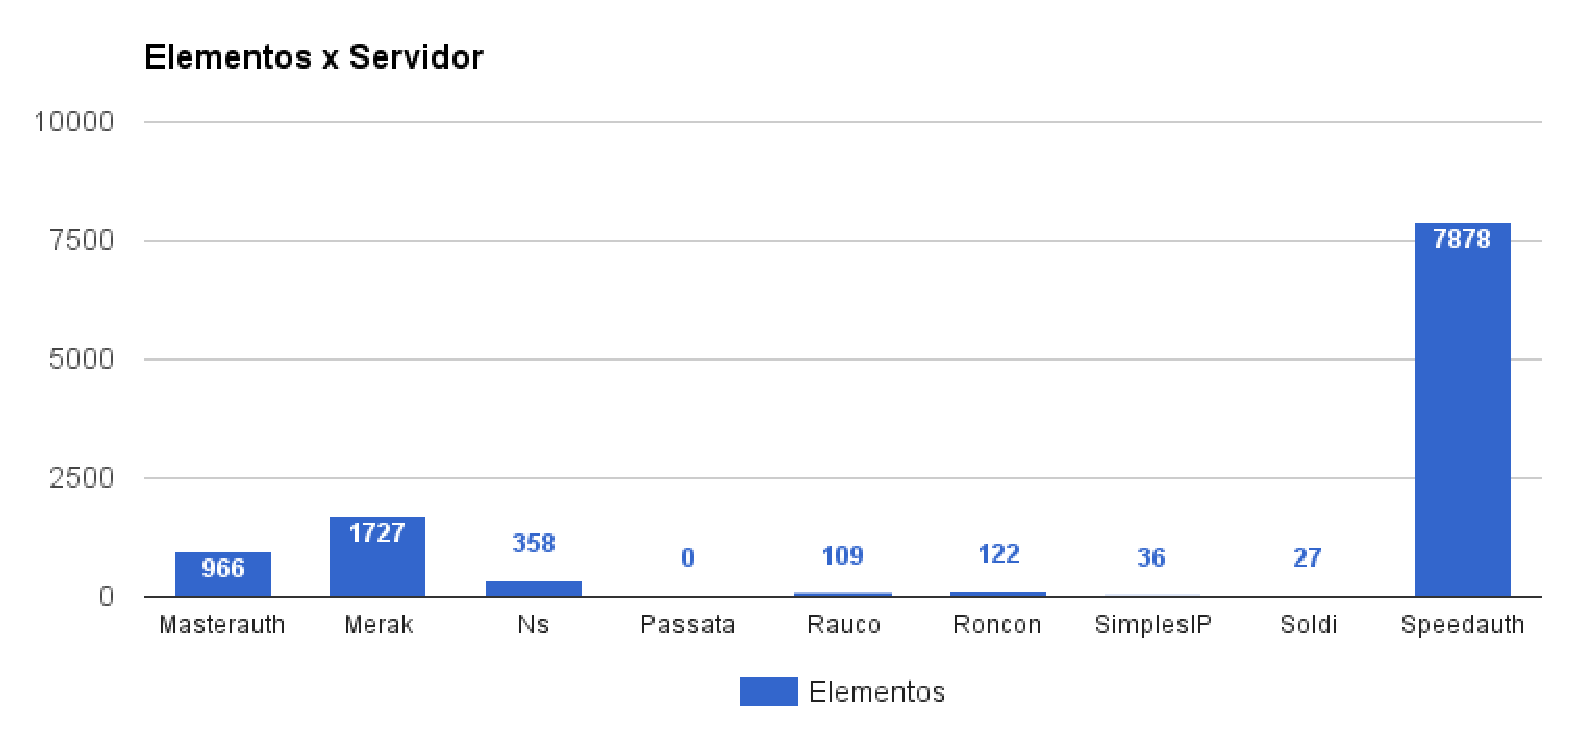
\includegraphics[width=430px]{img/servico_elemento.eps}
 \caption{Gráfico de comparação de elementos entre os principais servidores.}
 \label{fig:servico_elemento}
\end{figure}

 \item Sistemas da empresa e do provedor: o sistema do provedor é responsável pela maior parte das operações do provedor. De fato, esse sistema é
 responsável pela emissão de boletos e envio para clientes, atendimento de clientes, comunicação interna da empresa, vendas, ativações de novos 
 clientes, entre outros. Esse sistema não tem um impacto direto para os clientes, porém é fundamental para os funcionários da empresa e do provedor. 
 Caso haja uma indisponibilidade desses sistemas a maior parte dos funcionários ficarão impossibilitados de trabalhar.
 %, sendo que são aproximadamente 35 funcionários simultâneos (de acordo com a Figura \ref{fig:ejabberd_week}), isso poderia gerar um prejuizo elevado para a empresa e o provedor. 
 Pode-se aplicar o critério de número de requisições por segundo nesse serviço, sendo que o principal sistema do provedor, que está 
 executando sobre o servidor \textit{Soldi}, que recebe aproximadamente 3 requisições por segundo (Figura \ref{fig:soldi_week}). Além disso, a empresa 
 mantém outros 27 sistemas, de outros clientes, nesse mesmo servidor. Outro critério que aplica-se a esse serviço é o número de conexões \ac{TCP}, 
 onde pode-se observar que o servidor \textit{Soldi} está entre os mais relevantes, como pode ser observado na Figura \ref{fig:servico_tcp}.
 Sendo que essa figura compara os principais servidores da empresa através do critério de conexões \ac{TCP} que foi descrito anteriormente no 
 quarto critério;
 
\begin{figure}[h!]
 \centering
 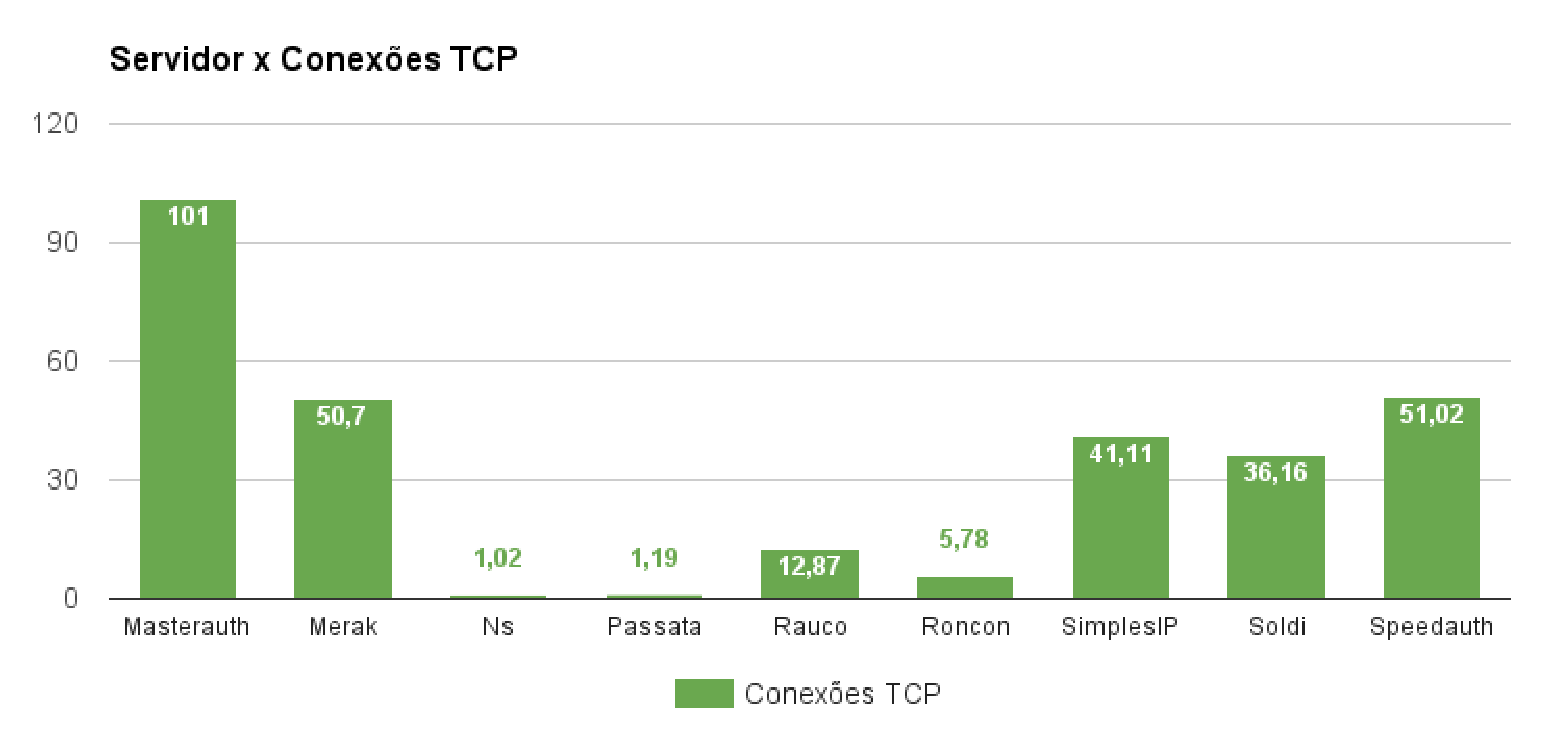
\includegraphics[width=430px]{img/servico_tcp.eps}
 \caption{Gráfico de comparação de conexões TCP entre os principais servidores.}
 \label{fig:servico_tcp}
\end{figure}

%\begin{figure}[h!]
% \centering
% 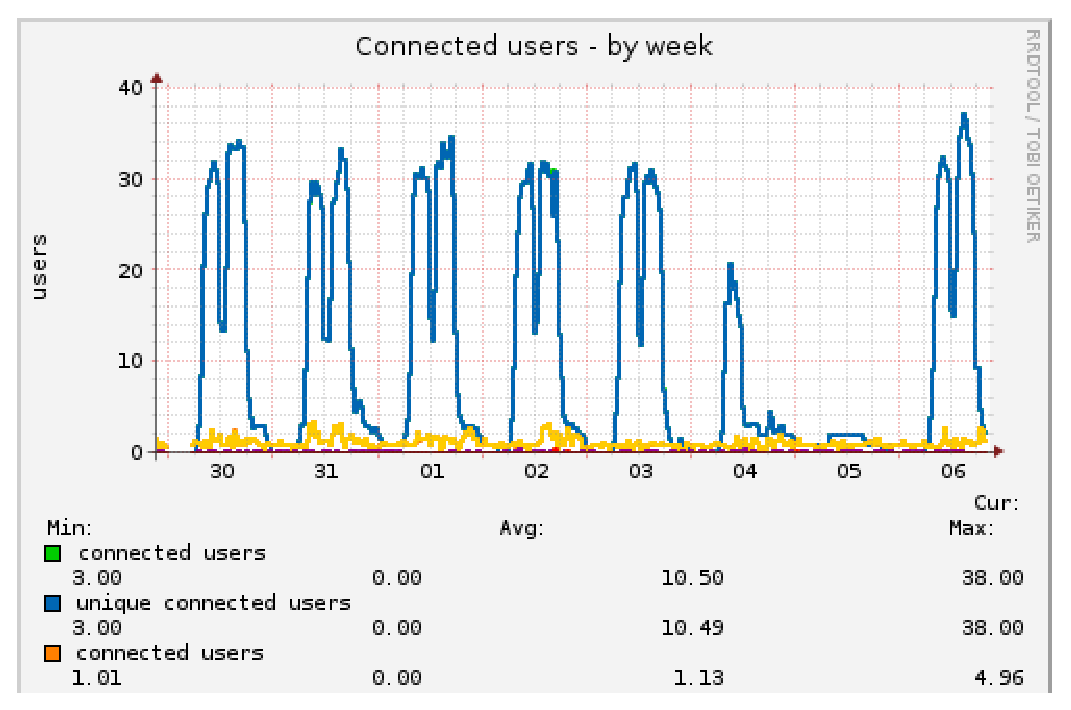
\includegraphics[width=310px]{img/ejabberd_week.eps}
% \caption{Gráfico usuários simultâneos de sistema.}
% \label{fig:ejabberd_week}
%\end{figure}

\begin{figure}[h!]
 \centering
 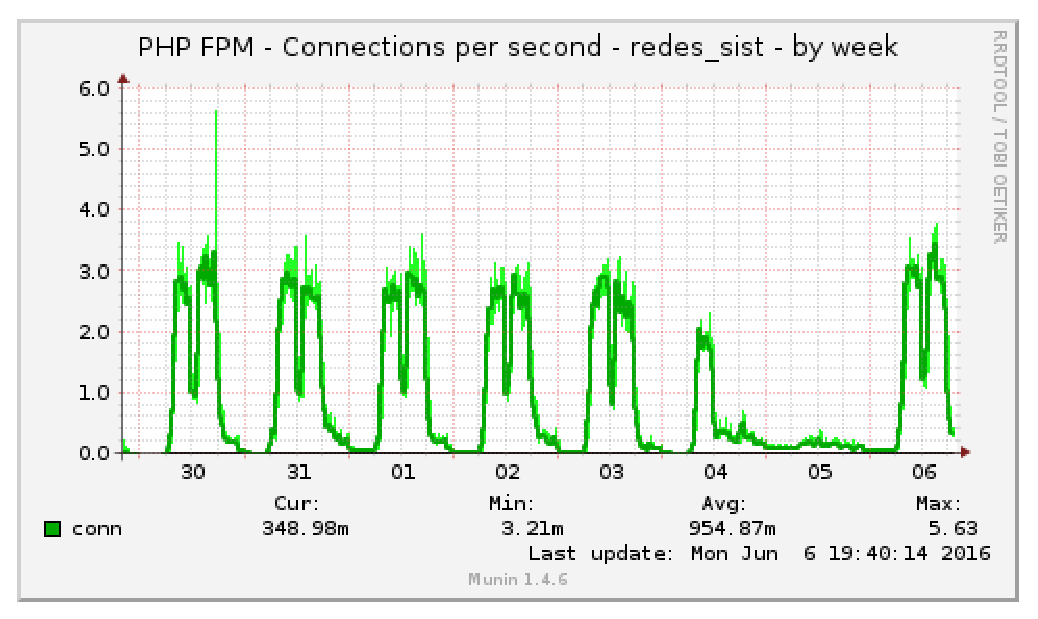
\includegraphics[width=310px]{img/soldi_week.eps}
 \caption{Gráfico de requisições por segundo do maior sistema.}
 \label{fig:soldi_week}
\end{figure}

 \item Telefonia: esse serviço tem relevância para a empresa e para o provedor, pois permite a comunicação entre os clientes e os funcionários, 
 ou seja, o servidor \textit{SimplesIP} é responsável por permitor o atendimento a clientes para fins de suporte técnico, comunicação interna entre 
 funcionários, comunicação com técnicos externos, vendas, cobranças a clientes, entre outros. Para quantificar, no mês de maio de 2016 a empresa 
 recebeu 15922 ligações, com duração total de 67 horas e 40 minutos, sendo que essas ligações foram recebidas por todos os setores do provedor e 
 também da empresa. Além disso, no mesmo mês foram efetuadas 674 ligações entre funcionários. O gráfico da Figura \ref{fig:simplesip_week} mostra 
 a quantidade de canais ativos no servidor de telefonia. Observa-se na Figura que são realizadas de 20 a 30 ligações durante o horário comercial, 
 das 08:00 às 12:00 e das 13:00 às 18:00. Outro critério que é relevante para este serviço é o número de conexões \ac{TCP} e o número de 
 transmissões \ac{UDP}, pois esse servidor também encontra-se entre os maiores. Ele pode ser observado na Figura \ref{fig:servico_tcp} e na Figura 
 \ref{fig:servico_udp}.
\end{itemize}

\begin{figure}[h!]
 \centering
 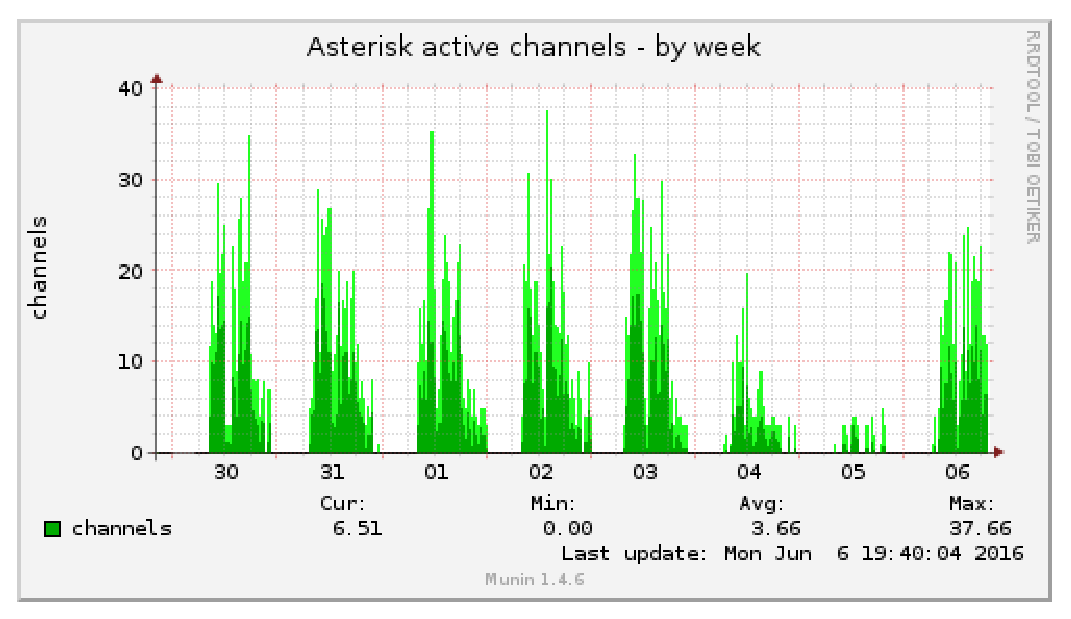
\includegraphics[width=310px]{img/simplesip_week.eps}
 \caption{Gráfico de requisições por segundo do maior sistema.}
 \label{fig:simplesip_week}
\end{figure}

Sobre os serviços descritos anteriormente, pode-se identificar quais máquinas virtuais deverão ser incluídas no 
ambiente de alta disponibilidade, sendo elas:
\begin{itemize}
 \item \textit{Passata}
 \item \textit{Speedauth}
 \item \textit{Masterauth}
 \item \textit{Soldi}
 \item \textit{SimplesIP}
\end{itemize}

\section{Proposta de solução}

O primeiro passo desta implementação é fazer uma reorganização das máquinas virtuais entre os servidores atuais, liberando assim o 
\textit{hardware} suficiente para possibilitar a implementação do ambiente de alta disponibilidade. (COMO??)

Após ter sido feito a reorganização das máquinas virtuais será iniciado a implementação, montando um ambiente com dois servidores e os 
configurando de uma forma que caso houver alguma falha, em um servidor físico ou no seu sistema operacional hospedeiro, as máquinas serão 
tranferidas para o outro servidor físico. 
A configuração dos servidores deverá ser de 11 \textit{cores} de processamento, 12 GB de memória e 156 GB de disco, sendo que essa configuração 
foi calculada a partir da soma dos recursos atuais das máquinas virtuais que possuem os serviços críticos, que foram apresentadas na Seção 
\ref{section:servcrit}.

As ferramentas necessárias para essa implementação podem ser divididas em dois grupos: ferramenta de replicação de dados 
(Seção \ref{section:toolrepl}) e ferramenta que faz o monitoramento e a tranferências das máquinas virtuais no caso de alguma falha 
(Seção \ref{section:toolcluster}).

\section{Ferramentas de replicação de dados}
\label{section:toolrepl}

Replicação de dados pode ser feita de diversas maneiras, pode ser a nível de aplicação ou até mesmo a nível de \textit{hardware}.
Dependendo do objetivo e da aplicação pode-se usar ferramentas como por exemplo o \textit{rsync}, que faz o sincronismo de dados de uma origem
para um destino. Sendo assim, não é possível utilizar essa ferramenta, pois ela não faz a replicação em tempo real, ou seja, se for necessário
utilizar os dados de destino ocorrerá perda de dados devido ao tempo de sincronismo. Outra forma de replicação é a de discos com \ac{RAID} 
por exemplo, essa solução é eficaz para garantir que o sistema não fique indisponível em caso de falha de discos\footnote{Lembrando que essa 
solução é utilizada no ambiente atual para aumentar a disponibilidade dos servidores}, porém não garante a disponibilidade quando \textit{software}
ou algum outro componente de \textit{hardware} falhar \cite{zaminhani2008}.

A solução de replicação ideal para esta implementação é um espelhamento de dados através da redes, sendo que essa solução permite a cópia dos 
dados para uma máquina remota em tempo real. Essa solução além de fazer a replicação dos dados, faz a redundância de todo \textit{hardware}.

A ferramenta escolhida para replicação de dados na solução de alta disponibilidade desse trabalho foi o \ac{DRBD}. Essa ferramenta é de código
aberto, e permite a replicação de dados de um dispositivo local em tempo real. 
APROFUNDAR AQUI OU NA IMPLEMENTAÇÂO? AQUI

figura??

% dispositivo primario e secundario zaminhani2008
% Segundo (ELLENBERG, 2007), a partir da versão 8 do DRBD é possível que,
%dependendo da aplicação, a execução ocorra em todos os nós do cluster
%simultaneamente (Ativo/Ativo). Para tornar isso possível é necessária a
%utilização de um sistema de arquivos exclusivo para cluster, como o OCFS2 6 e o
%GFS 7 por exemplo. Como a abordagem deste trabalho é cluster de alta
%disponibilidade, a utilização do DRBD no modo Ativo/Ativo não será discutida.

\section{Ferramentas de gerenciamento de cluster}
\label{section:toolcluster}

Para ser possível implementar uma solução de alta disponibilidade é necessário uma ferramenta que monitora os recursos, fazendo a detecção e
recuperação do serviço utilizando mensagens entre os servidores, que é denominada como um \textit{cluster} \cite{perkov2011}. 
Pode-se definir \textit{cluster} como um grupo de computadores interligador por rede com o objetivo de aumentar o desempenho ou disponibilidade
de um serviço \cite{freitas2005}.

Essas ferramentas de gerenciamento de \textit{cluster} permitem detecção de falhas a nível de nó e a nível de recursos, ou seja, pode detectar
falhas de \textit{hardware} e falhas de serviços (recursos).
Elas são conhecidas como \ac{CRM}, cujo sua função é fazer a gerência de recursos de um \textit{cluster}.

O \ac{CRM} escolhido para gerenciar o ambiente foi o \textit{Pacemaker} ...
Outras ferramentas CRM (nao tenho certeza?):
Microsoft com+ cluster ???
ZS3-2 Clustering ???

O \textit{Pacemaker} \cite{pacemaker}, que pode ser definido como uma ferramenta de detecção e recuperação de falhas a nível de 
serviço \cite{perkov2011}. Essa ferramenta é um projeto de código aberto mantido pela \cite{clusterlabs}, 
e teve origem com a necessidade de criar um gerenciador de recursos para a ferramenta \textit{Heartbeat} \cite{heartbeat}. 

O \ac{CRM} \textit{Pacemaker} possui algumas características que estão listadas abaixo:
\begin{itemize}
 \item Inicia e para serviços, como, por exemplo, servidor \textit{web}, interface de rede, entre outros;
 \item Replica a configuração do \textit{cluster} para todos os nós de forma transparente, com isso a configuração de todo o \textit{cluster} 
 pode ser feita em qualquer nó;
 \item ...
\end{itemize}

A arquitetura do \textit{Pacemaker} pode ser dividida em três partes:
\begin{itemize}
 \item 
\end{itemize}

Esse \ac{CRM} funciona em conjunto com ferramentas de troca de mensagens ...

\begin{figure}[h!]
 \centering
 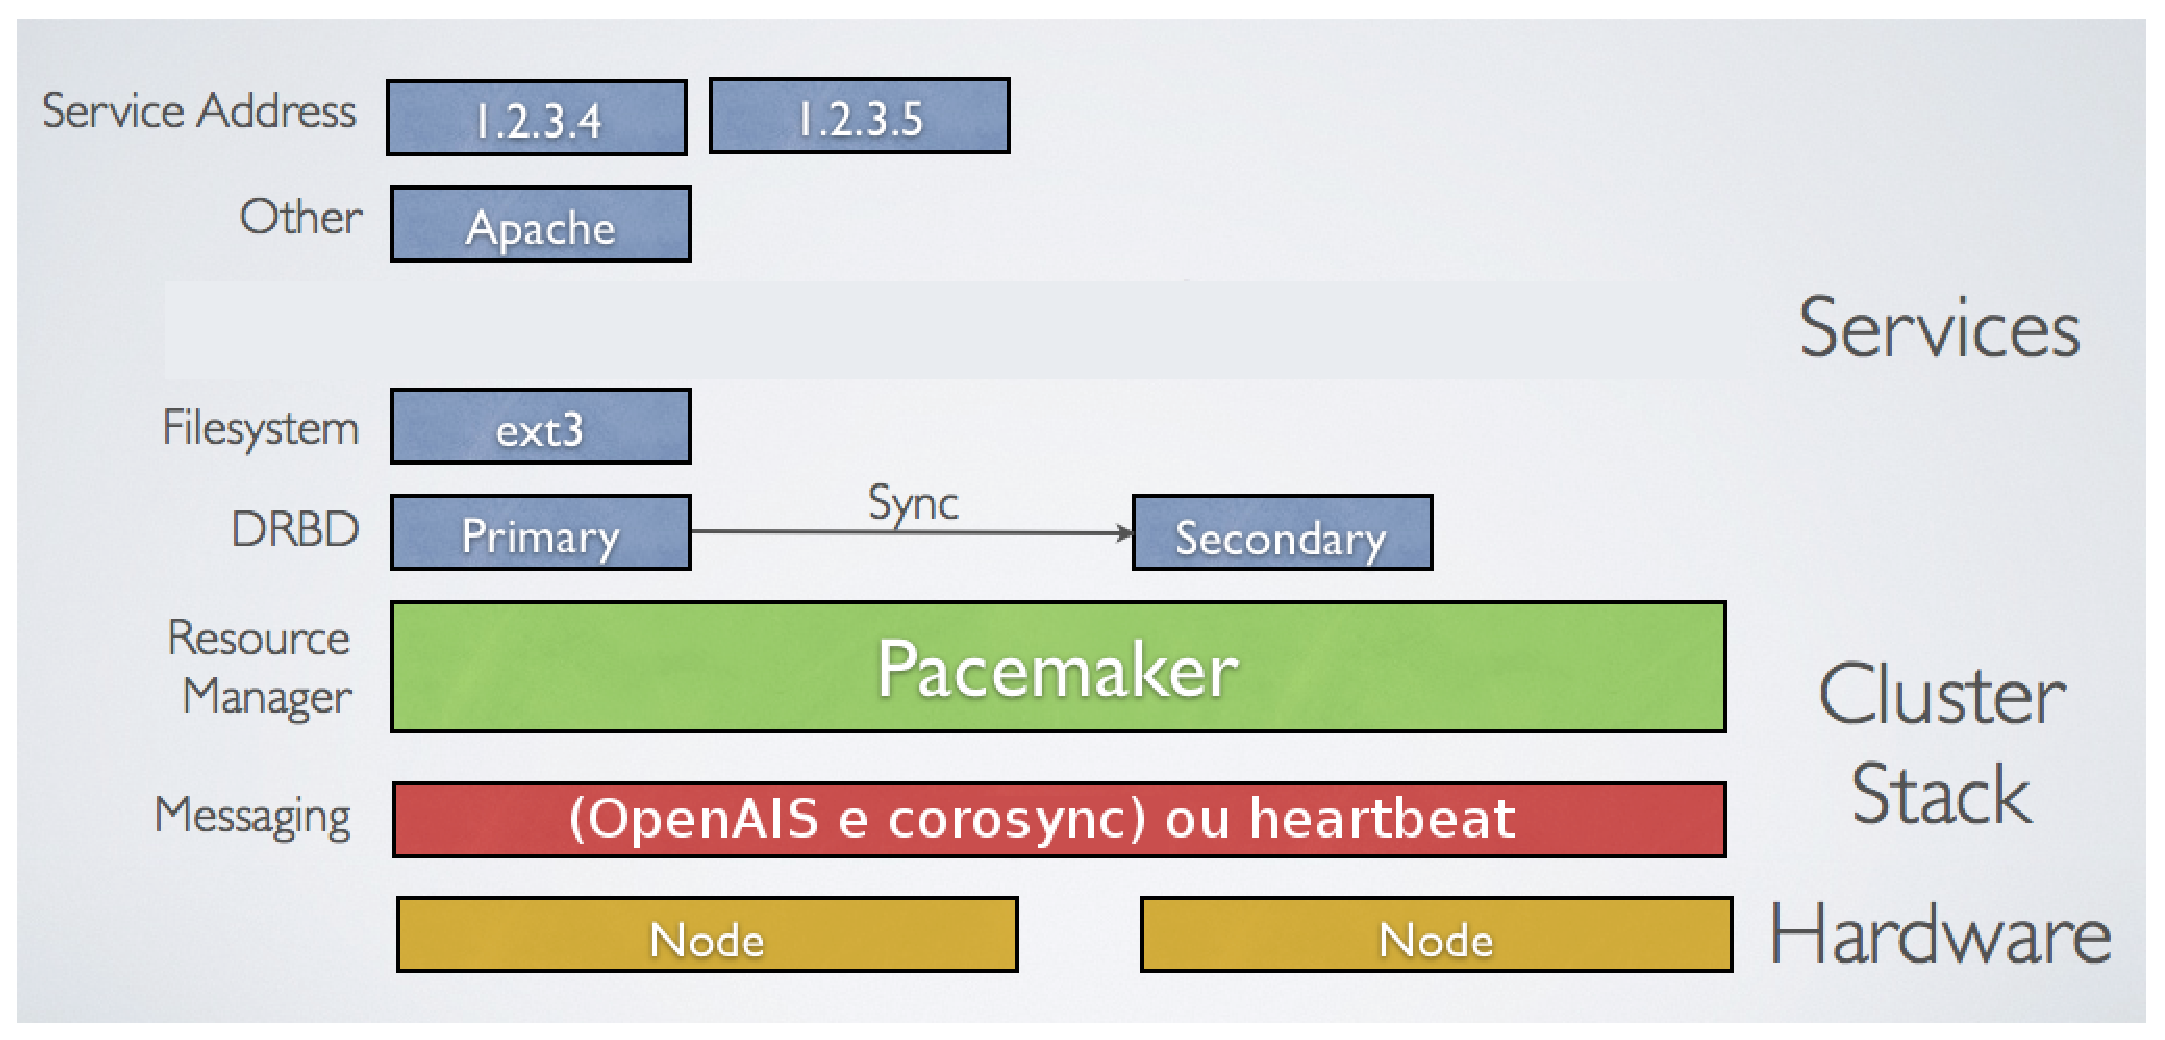
\includegraphics[width=300px]{img/pacemaker_tools.eps}
 \caption{Pacemaker estrutura}
 Fonte: \citet{pacemaker}
 \label{fig:pacemaker_tools}
\end{figure}

O \textit{Heartbeat} é um mecanismo que faz envio de mensagens entre os nós do \textit{cluster} com objetivo de notificar esse 
\textit{cluster} quando houver alguma alteração de estado dos recursos ou dos nós \cite{clusterlabs}. O \textit{Heartbeat} é um subprojeto do
\textit{Linux-HA} \cite{linuxha}.

As ferramentas \textit{OpenAIS} e \textit{Corosync} ...

\cite{clusterlabs}:
Corosync provides pacemaker:
a mechanism to reliably send messages between nodes,
notifications when machines appear and disappear
a list of machines that are up that is consistent throughout the cluster 
Heartbeat provides:
a mechanism to reliably send messages between nodes,
notifications when machines appear and disappear
a list of machines that are up that is consistent throughout the cluster 
--
http://serverfault.com/questions/269831/relation-between-heartbeat-openais-corosync
well i reached answer on myself! clustering include two part:
1.cluster resource management
2.infrastructure with massaging layer
legacy heartbeat is broken into heartbeat message layer and pacemaker so pacemaker is CRM.
and we have two option on message layer:heartbeat,openais. openais/corosync is preferred as: http://comments.gmane.org/gmane.linux.highavailability.user/32355
There are, however, features in Pacemaker that require OpenAIS which will work only with Corosync, not Heartbeat. Those features are concerned 
with the distributed lock managers used by cLVM (but not regular LVM), GFS/GFS2, and OCFS2. If you need that functionality, you must select 
OpenAIS/Corosync. If you do not, you're free to choose.
as: http://www.clusterlabs.org/wiki/FAQ
Originally Corosync and OpenAIS were the same thing. Then they split into two parts... the core messaging and membership capabilities are now 
called Corosync, and OpenAIS retained the layer containing the implementation of the AIS standard.
Pacemaker itself only needs the Corosync piece in order to function, however some of the applications it can manage (such as OCFS2 and GFS2) 
require the OpenAIS layer as well.
so i went to openais/corosync and integrate it with pacemaker.
--
There are, however, features in Pacemaker that require OpenAIS which
will work only with Corosync, not Heartbeat. Those features are
concerned with the distributed lock managers used by cLVM (but not
regular LVM), GFS/GFS2, and OCFS2. If you need that functionality, you
must select OpenAIS/Corosync.

Pacemaker itself only needs the Corosync piece in order to function, however some of the applications it can manage 
(such as OCFS2 and GFS2) require the OpenAIS layer as well. 


Explicar live migration \ref{fig:vms_migration}
%http://www.aliancatecnologia.com/conteudo/2015/05/quatro-estrategias-de-protecao-para-seu-ambiente-virtual/

\begin{figure}[h!]
 \centering
 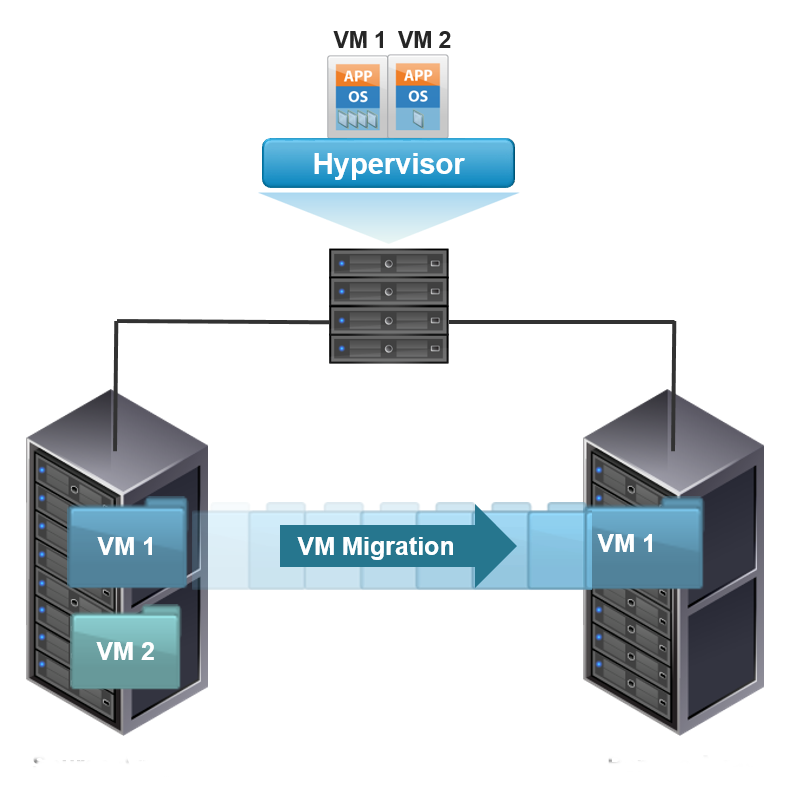
\includegraphics[width=300px]{img/vms_migration.eps}
 \caption{Live migration}
 Fonte: \citet{spaniol2015}
 \label{fig:vms_migration}
\end{figure}

Fazendo testes e valiando...

%reorganização de vms
%ferramentas selecionadas, colocar motivo para escolher e citar ferramentas parecidas
%muitos servicos, melhor solucao utilizar 2 servidores para fazer redundancia
%em caso de falha de um servidor fisico...
%ferramentas open source...
%colocar a disponibilidade do nagios do ano passado?
